\section{Evaluation events}
\label{evaluations}
Figure~\ref{fig:eval} depicts the concepts involved in creating a result by
evaluating a validating or aggregating expression. Conceptually, the \textsf{data}
consists of values bound to variable names. The \emph{expression} denotes, using
a fixed set of syntax rules, a computation on variables present in the \emph{data}.
In the \emph{evaluation} event, the following activities take place
\begin{enumerate}[noitemsep]
\item Read the expression and check whether it is valid syntax. If not: stop execution.
\item Parse the expression: substitute variable names with the corresponding values
stored in \emph{data}.
\item Evaluate the expression, creating the \emph{result}.
\end{enumerate}
As a demonstration that both validation and aggregation fit in this description,
consider the following two examples.
%
\begin{figure}
\centering
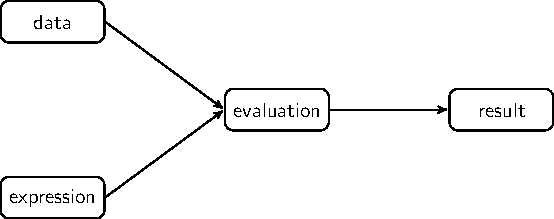
\includegraphics[width=0.8\textwidth]{fig/eval.pdf}
\caption{Concepts involved in evaluating a (validating or aggregating) expression.}
\label{fig:eval}
\end{figure}

\begin{example}
Consider the expression
\begin{align*}
\texttt{age >= 0}
\end{align*}
and a data record given by
\begin{center}
\begin{tabular}{lll}
Name & Age & Sex \\
\hline
Joe  & 17  & male
\end{tabular}
\end{center}
In the first step, the evaluator reads in the expression and approves it after
checking with the syntax. In the second step, the variable names are identified
and replaced with matching values from the dataset. This yields \code{17 >= 0}.
Finally, in the third step the proposition \code{17 >= 0} is evaluated and the
result returned.
\end{example}

\begin{example} Consider the following table of validation results (we use
1 for \waar{} and 0 for \onwaar{}).
\begin{center}
\begin{tabular}{lr}
Name  & validation\_result \\
\hline
Alice & 1    \\
Bob   & 1    \\
Carol & 0    \\
\end{tabular}
\end{center}
The expression counting the number of passes is given by
\begin{align*}
\texttt{sum(validation\_result)}.
\end{align*}
In the first step the evaluator reads in the expression and approves it after
checking with the syntax. In the second step, the variable names are identified
and the expression is expanded\footnote{Conceptually of course. In practice
accumulation will be more efficient.} to \code{1 + 1 + 0}.  This expression is
then evaluated and its result returned.
\end{example}
Obviously, to identify the meaning of a result, both the input data and the
expression used must be known. However, the value of the final result may also
depend on the (version of) the evaluator. Especially since the Handbook on
Validation explicitly includes the possibility of validation being done by
expert review. In that case, the `expression' may be a manual or handbook with
recommendations on evaluating a certain dataset and the result is a validity
assessment by an expert. But even in the case of formalized expressions,
interpreters may differ. Formal programming syntax standards often leave
certain details to interpreter developers. This inevitably leads to
platform-dependent results. 

It is therefore proposed here to include metadata elements that identify data,
expression, and the evaluating event for all results reported in a validation
report, whether they are aggregates or validation results. Since validation
results have a particular type and meaning that differs from aggregation
results it will be useful to differentiate their metadata as well.









